\section{Project Overview}
Note: the wavemaker reference manual is available at (http://www.wavemaker.com/learn/documentation-reference/ ). 

Wavemaker provides a set of different project views, see Figure~\ref{fig:workspace}. The \textbf{design view}, accessed by the button inside the green circle, allows users to design the web interface using a drag-and-drop approach. At any time users can switch to the \textbf{script view}, by clicking on the button inside the blue circle, to add event-handlers in javascript. Wavemaker is using angularjs which is a javascript library. To add an \textbf{event handler} to a control in the UI, use the button (inside the red circle) with hand-like caption. To edit an existing \textbf{control properties}, use the button (inside the black circle) with the palette-like caption.  
To integrate a \textbf{new service}, click on import (inside the brown circle) then click new web service. Follow the steps in the wizard to define the new service with its parameters. To update an existing service, click on services link (inside the orange circle) on the left-hand side. NEMO has multiple design views, to switch to another view click on the button \textbf{select view} inside the purple circle. Please read wavemaker manual for additional functionality.

\begin{figure}[H]
\centering
%\label{fig:ebola-kshell-not-effective}
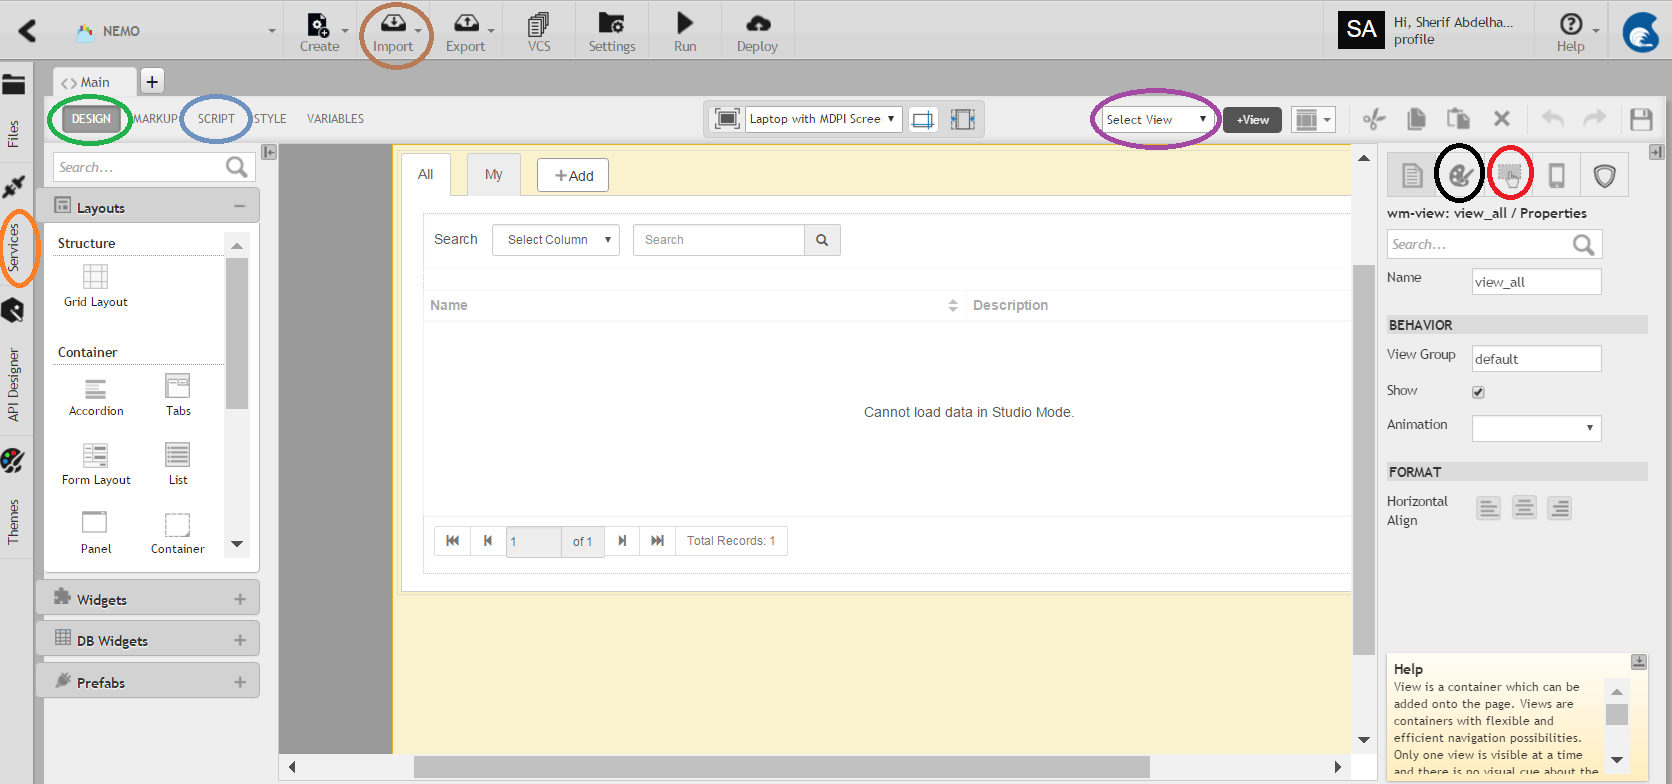
\includegraphics[trim = 0.0in 0.0in 0.0in 0.0in,scale=0.5]{workspace}
\caption{
Project workspace in Wavemaker. Each circle refer to different functionality.
}   %   
\label{fig:workspace}
\end{figure}